\documentclass{article}\usepackage[]{graphicx}\usepackage[]{color}
%% maxwidth is the original width if it is less than linewidth
%% otherwise use linewidth (to make sure the graphics do not exceed the margin)
\makeatletter
\def\maxwidth{ %
  \ifdim\Gin@nat@width>\linewidth
    \linewidth
  \else
    \Gin@nat@width
  \fi
}
\makeatother

\definecolor{fgcolor}{rgb}{0.345, 0.345, 0.345}
\newcommand{\hlnum}[1]{\textcolor[rgb]{0.686,0.059,0.569}{#1}}%
\newcommand{\hlstr}[1]{\textcolor[rgb]{0.192,0.494,0.8}{#1}}%
\newcommand{\hlcom}[1]{\textcolor[rgb]{0.678,0.584,0.686}{\textit{#1}}}%
\newcommand{\hlopt}[1]{\textcolor[rgb]{0,0,0}{#1}}%
\newcommand{\hlstd}[1]{\textcolor[rgb]{0.345,0.345,0.345}{#1}}%
\newcommand{\hlkwa}[1]{\textcolor[rgb]{0.161,0.373,0.58}{\textbf{#1}}}%
\newcommand{\hlkwb}[1]{\textcolor[rgb]{0.69,0.353,0.396}{#1}}%
\newcommand{\hlkwc}[1]{\textcolor[rgb]{0.333,0.667,0.333}{#1}}%
\newcommand{\hlkwd}[1]{\textcolor[rgb]{0.737,0.353,0.396}{\textbf{#1}}}%

\usepackage{framed}
\makeatletter
\newenvironment{kframe}{%
 \def\at@end@of@kframe{}%
 \ifinner\ifhmode%
  \def\at@end@of@kframe{\end{minipage}}%
  \begin{minipage}{\columnwidth}%
 \fi\fi%
 \def\FrameCommand##1{\hskip\@totalleftmargin \hskip-\fboxsep
 \colorbox{shadecolor}{##1}\hskip-\fboxsep
     % There is no \\@totalrightmargin, so:
     \hskip-\linewidth \hskip-\@totalleftmargin \hskip\columnwidth}%
 \MakeFramed {\advance\hsize-\width
   \@totalleftmargin\z@ \linewidth\hsize
   \@setminipage}}%
 {\par\unskip\endMakeFramed%
 \at@end@of@kframe}
\makeatother

\definecolor{shadecolor}{rgb}{.97, .97, .97}
\definecolor{messagecolor}{rgb}{0, 0, 0}
\definecolor{warningcolor}{rgb}{1, 0, 1}
\definecolor{errorcolor}{rgb}{1, 0, 0}
\newenvironment{knitrout}{}{} % an empty environment to be redefined in TeX

\usepackage{alltt}

\usepackage[margin = 0.5in]{geometry}
\usepackage{float, enumitem}
\usepackage{graphicx}
\usepackage{amsmath}

\setlength{\topsep}{0pt}
\setlength{\parskip}{0pt}
\setlength{\partopsep}{1pt}

\renewcommand\thesubsection{\thesection (\alph{subsection})}
\IfFileExists{upquote.sty}{\usepackage{upquote}}{}
\begin{document}

\title{ASSIGNMENT 8}
\author{Brandon Lampe \\ STAT 527 \\ Advanced Data Analysis I}
\maketitle



\section{Gas milage and automobile horsepower:}
\subsection{(10 pts) Scatter Plots of Data.}

\begin{knitrout}
\definecolor{shadecolor}{rgb}{0.969, 0.969, 0.969}\color{fgcolor}\begin{kframe}
\begin{alltt}
\hlcom{# # read the table in as a data.frame}
\hlcom{# # cars <- read.table("http://statacumen.com/teach/ADA1/ADA1_HW_08_F14-1.txt", header=TRUE)}
\hlcom{#}
\hlcom{# # write.table(cars, file = "/Users/Lampe/Documents/UNM_Courses/STAT-527_ADAI_ERHARDT/HW08/cars.txt",}
\hlcom{# #       sep = ",", col.names = TRUE)}

\hlstd{cars} \hlkwb{<-} \hlkwd{read.csv}\hlstd{(}\hlstr{"/Users/Lampe/Documents/UNM_Courses/STAT-527_ADAI_ERHARDT/HW08/cars.txt"}\hlstd{,} \hlkwc{header} \hlstd{=} \hlnum{TRUE}\hlstd{)}
\end{alltt}
\end{kframe}
\end{knitrout}

\begin{knitrout}
\definecolor{shadecolor}{rgb}{0.969, 0.969, 0.969}\color{fgcolor}\begin{kframe}
\begin{alltt}
\hlcom{# plot mpg = f(hp)}
\hlstd{p1a} \hlkwb{<-} \hlkwd{ggplot}\hlstd{(cars,} \hlkwd{aes}\hlstd{(}\hlkwc{x} \hlstd{= hp,} \hlkwc{y} \hlstd{= mpg))}
\hlstd{p1a} \hlkwb{<-} \hlstd{p1a} \hlopt{+} \hlkwd{geom_point}\hlstd{()}
\hlstd{p1a} \hlkwb{<-} \hlstd{p1a} \hlopt{+} \hlkwd{labs}\hlstd{(}\hlkwc{y} \hlstd{=} \hlstr{"Miles Per Gallon"}\hlstd{,} \hlkwc{x} \hlstd{=} \hlstr{"Horsepower"}\hlstd{)}
\hlstd{p1a} \hlkwb{<-} \hlstd{p1a} \hlopt{+} \hlkwd{geom_smooth}\hlstd{(}\hlkwc{method} \hlstd{= lm,} \hlkwc{se} \hlstd{=} \hlnum{FALSE}\hlstd{)}
\hlstd{p1a}
\end{alltt}
\end{kframe}

{\centering 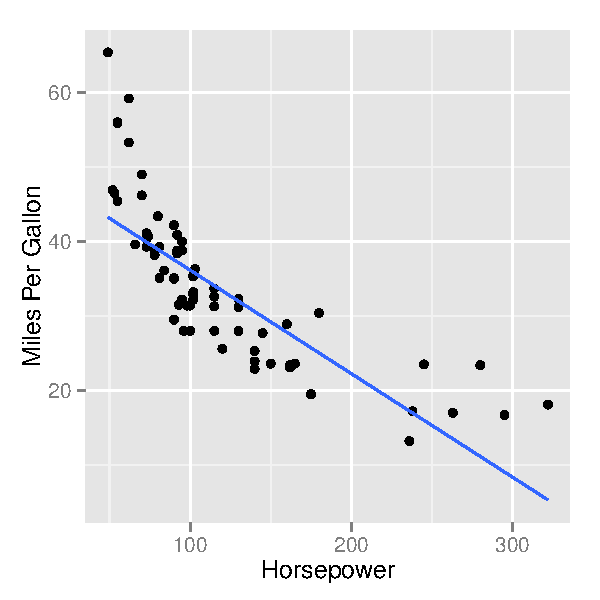
\includegraphics[width=\maxwidth]{figure/1a-1} 

}


\begin{kframe}\begin{alltt}
\hlstd{lm.mpg.hp} \hlkwb{<-} \hlkwd{lm}\hlstd{(mpg} \hlopt{~} \hlstd{hp,} \hlkwc{data} \hlstd{= cars)}
\hlstd{sum.lm.mpg.hp} \hlkwb{<-} \hlkwd{summary}\hlstd{(lm.mpg.hp)}
\hlkwd{summary}\hlstd{(lm.mpg.hp)}
\end{alltt}
\begin{verbatim}
## 
## Call:
## lm(formula = mpg ~ hp, data = cars)
## 
## Residuals:
##     Min      1Q  Median      3Q     Max 
## -8.7198 -4.1224 -0.9077  3.1009 22.1461 
## 
## Coefficients:
##             Estimate Std. Error t value Pr(>|t|)    
## (Intercept) 50.06608    1.56949   31.90   <2e-16 ***
## hp          -0.13902    0.01207  -11.52   <2e-16 ***
## ---
## Signif. codes:  0 '***' 0.001 '**' 0.01 '*' 0.05 '.' 0.1 ' ' 1
## 
## Residual standard error: 6.174 on 80 degrees of freedom
## Multiple R-squared:  0.6239,	Adjusted R-squared:  0.6192 
## F-statistic: 132.7 on 1 and 80 DF,  p-value: < 2.2e-16
\end{verbatim}
\end{kframe}
\end{knitrout}

\begin{knitrout}
\definecolor{shadecolor}{rgb}{0.969, 0.969, 0.969}\color{fgcolor}\begin{kframe}
\begin{alltt}
\hlstd{cars}\hlopt{$}\hlstd{log_hp} \hlkwb{<-} \hlkwd{log}\hlstd{(cars}\hlopt{$}\hlstd{hp)}
\hlstd{cars}\hlopt{$}\hlstd{log_mpg} \hlkwb{<-} \hlkwd{log}\hlstd{(cars}\hlopt{$}\hlstd{mpg)}
\hlstd{cars}\hlopt{$}\hlstd{log_wt} \hlkwb{<-} \hlkwd{log}\hlstd{(cars}\hlopt{$}\hlstd{wt)}

\hlstd{p1b} \hlkwb{<-} \hlkwd{ggplot}\hlstd{(cars,} \hlkwd{aes}\hlstd{(}\hlkwc{x} \hlstd{= log_hp,} \hlkwc{y} \hlstd{= mpg))}
\hlstd{p1b} \hlkwb{<-} \hlstd{p1b} \hlopt{+} \hlkwd{geom_point}\hlstd{()}
\hlstd{p1b} \hlkwb{<-} \hlstd{p1b} \hlopt{+} \hlkwd{labs}\hlstd{(}\hlkwc{y} \hlstd{=} \hlstr{"Miles Per Gallon"}\hlstd{,} \hlkwc{x} \hlstd{=} \hlstr{"Log Horsepower"}\hlstd{)}
\hlstd{p1b} \hlkwb{<-} \hlstd{p1b} \hlopt{+} \hlkwd{geom_smooth}\hlstd{(}\hlkwc{method} \hlstd{= lm,} \hlkwc{se} \hlstd{=} \hlnum{FALSE}\hlstd{)}
\hlstd{p1b}
\end{alltt}
\end{kframe}

{\centering 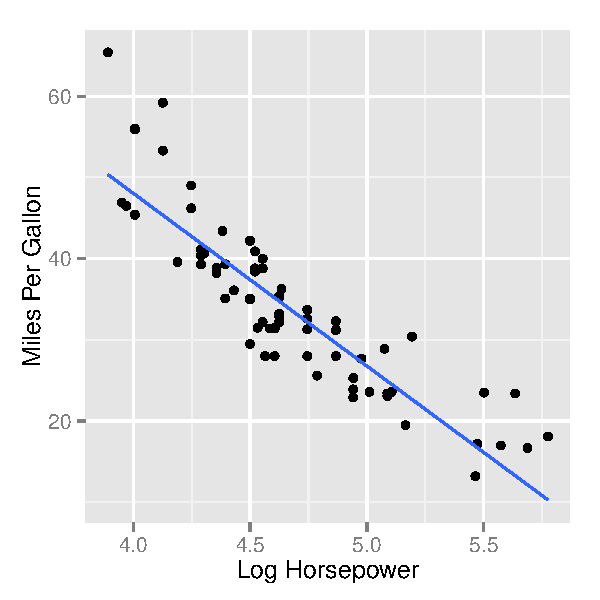
\includegraphics[width=\maxwidth]{figure/1a2-1} 

}


\begin{kframe}\begin{alltt}
\hlstd{p1c} \hlkwb{<-} \hlkwd{ggplot}\hlstd{(cars,} \hlkwd{aes}\hlstd{(}\hlkwc{x} \hlstd{= hp,} \hlkwc{y} \hlstd{= log_mpg))}
\hlstd{p1c} \hlkwb{<-} \hlstd{p1c} \hlopt{+} \hlkwd{geom_point}\hlstd{()}
\hlstd{p1c} \hlkwb{<-} \hlstd{p1c} \hlopt{+} \hlkwd{labs}\hlstd{(}\hlkwc{y} \hlstd{=} \hlstr{"Log Miles Per Gallon"}\hlstd{,} \hlkwc{x} \hlstd{=} \hlstr{"Horsepower"}\hlstd{)}
\hlstd{p1c} \hlkwb{<-} \hlstd{p1c} \hlopt{+} \hlkwd{geom_smooth}\hlstd{(}\hlkwc{method} \hlstd{= lm,} \hlkwc{se} \hlstd{=} \hlnum{FALSE}\hlstd{)}
\hlstd{p1c}
\end{alltt}
\end{kframe}

{\centering 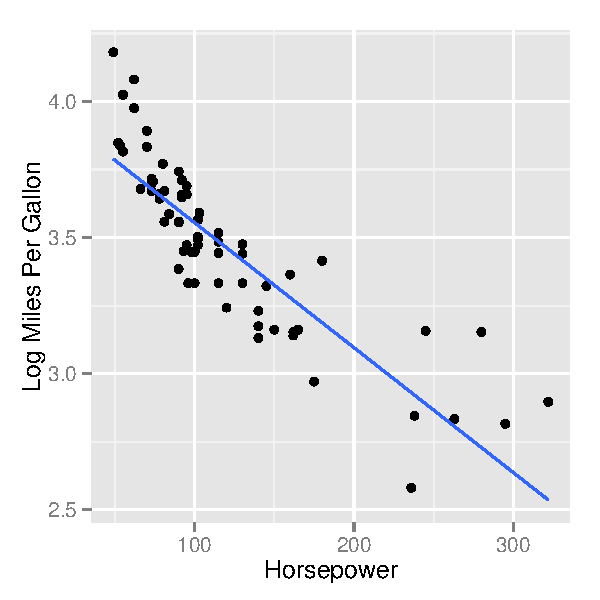
\includegraphics[width=\maxwidth]{figure/1a2-2} 

}


\begin{kframe}\begin{alltt}
\hlstd{lm.mpg.loghp} \hlkwb{<-} \hlkwd{lm}\hlstd{(mpg} \hlopt{~} \hlstd{log_hp,} \hlkwc{data} \hlstd{= cars)}
\hlstd{sum.lm.mpg.loghp} \hlkwb{<-} \hlkwd{summary}\hlstd{(lm.mpg.loghp)}
\hlkwd{summary}\hlstd{(lm.mpg.loghp)}
\end{alltt}
\begin{verbatim}
## 
## Call:
## lm(formula = mpg ~ log_hp, data = cars)
## 
## Residuals:
##     Min      1Q  Median      3Q     Max 
## -8.0422 -2.9050 -0.9174  2.5020 15.0468 
## 
## Coefficients:
##             Estimate Std. Error t value Pr(>|t|)    
## (Intercept)  133.169      5.855   22.75   <2e-16 ***
## log_hp       -21.279      1.249  -17.04   <2e-16 ***
## ---
## Signif. codes:  0 '***' 0.001 '**' 0.01 '*' 0.05 '.' 0.1 ' ' 1
## 
## Residual standard error: 4.678 on 80 degrees of freedom
## Multiple R-squared:  0.784,	Adjusted R-squared:  0.7813 
## F-statistic: 290.5 on 1 and 80 DF,  p-value: < 2.2e-16
\end{verbatim}
\begin{alltt}
\hlstd{lm.logmpg.hp} \hlkwb{<-} \hlkwd{lm}\hlstd{(log_mpg} \hlopt{~} \hlstd{hp,} \hlkwc{data} \hlstd{= cars)}
\hlstd{sum.lm.logmpg.hp} \hlkwb{<-} \hlkwd{summary}\hlstd{(lm.logmpg.hp)}
\hlkwd{summary}\hlstd{(lm.logmpg.hp)}
\end{alltt}
\begin{verbatim}
## 
## Call:
## lm(formula = log_mpg ~ hp, data = cars)
## 
## Residuals:
##      Min       1Q   Median       3Q      Max 
## -0.35003 -0.10508 -0.00974  0.07242  0.42440 
## 
## Coefficients:
##               Estimate Std. Error t value Pr(>|t|)    
## (Intercept)  4.0132294  0.0401238  100.02   <2e-16 ***
## hp          -0.0045889  0.0003085  -14.87   <2e-16 ***
## ---
## Signif. codes:  0 '***' 0.001 '**' 0.01 '*' 0.05 '.' 0.1 ' ' 1
## 
## Residual standard error: 0.1578 on 80 degrees of freedom
## Multiple R-squared:  0.7344,	Adjusted R-squared:  0.7311 
## F-statistic: 221.2 on 1 and 80 DF,  p-value: < 2.2e-16
\end{verbatim}
\end{kframe}
\end{knitrout}

\begin{knitrout}
\definecolor{shadecolor}{rgb}{0.969, 0.969, 0.969}\color{fgcolor}\begin{kframe}
\begin{alltt}
\hlstd{p1d} \hlkwb{<-} \hlkwd{ggplot}\hlstd{(cars,} \hlkwd{aes}\hlstd{(}\hlkwc{x} \hlstd{= log_hp,} \hlkwc{y} \hlstd{= log_mpg))}
\hlstd{p1d} \hlkwb{<-} \hlstd{p1d} \hlopt{+} \hlkwd{geom_point}\hlstd{()}
\hlstd{p1d} \hlkwb{<-} \hlstd{p1d} \hlopt{+} \hlkwd{labs}\hlstd{(}\hlkwc{y} \hlstd{=} \hlstr{"Log Miles Per Gallon"}\hlstd{,} \hlkwc{x} \hlstd{=} \hlstr{"Log Horsepower"}\hlstd{)}
\hlstd{p1d} \hlkwb{<-} \hlstd{p1d} \hlopt{+} \hlkwd{geom_smooth}\hlstd{(}\hlkwc{method} \hlstd{= lm)}
\hlstd{p1d}
\end{alltt}
\end{kframe}

{\centering 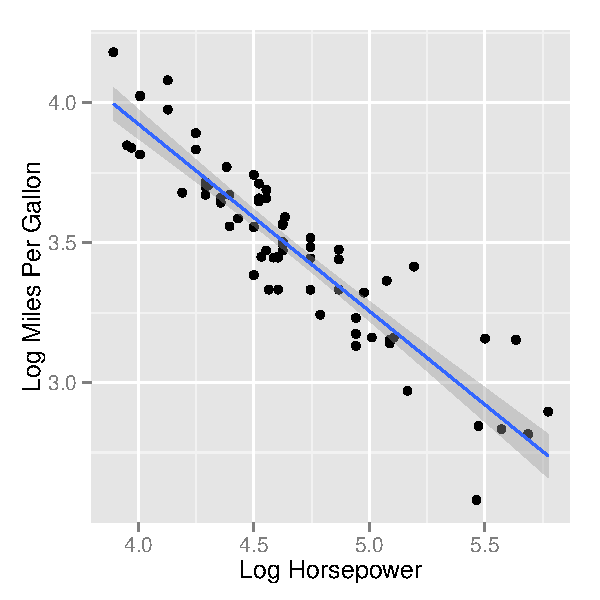
\includegraphics[width=\maxwidth]{figure/1a3-1} 

}


\begin{kframe}\begin{alltt}
\hlstd{lm.logmpg.loghp} \hlkwb{<-} \hlkwd{lm}\hlstd{(log_mpg} \hlopt{~} \hlstd{log_hp,} \hlkwc{data} \hlstd{= cars)}
\hlstd{sum.lm.logmpg.loghp} \hlkwb{<-} \hlkwd{summary}\hlstd{(lm.logmpg.loghp)}
\hlkwd{summary}\hlstd{(lm.logmpg.loghp)}
\end{alltt}
\begin{verbatim}
## 
## Call:
## lm(formula = log_mpg ~ log_hp, data = cars)
## 
## Residuals:
##      Min       1Q   Median       3Q      Max 
## -0.36502 -0.08179 -0.02332  0.09198  0.32183 
## 
## Coefficients:
##             Estimate Std. Error t value Pr(>|t|)    
## (Intercept)  6.59911    0.15492   42.60   <2e-16 ***
## log_hp      -0.66874    0.03304  -20.24   <2e-16 ***
## ---
## Signif. codes:  0 '***' 0.001 '**' 0.01 '*' 0.05 '.' 0.1 ' ' 1
## 
## Residual standard error: 0.1238 on 80 degrees of freedom
## Multiple R-squared:  0.8366,	Adjusted R-squared:  0.8346 
## F-statistic: 409.7 on 1 and 80 DF,  p-value: < 2.2e-16
\end{verbatim}
\end{kframe}
\end{knitrout}

Based on these graphical representations of data, a log-log transformation of the data (both
x and y) is most appropriate for a straight-line regression.  Additionally, the R-squared value for the log-log transformation is the highest of the four fits at 0.84, which means the log(mpg) vs log(hp) transformation most closely follows a straight-line regression model.

\subsection{(10 pts) Using the more appropriate of the two pairs of variables from (a), that is original or log-
transformed variables, fit a simple linear regression model.}

The log-log transformation was determined to be the most appropriate form for a linear regression model, results of this model and the data are shown below.  A summary of this regression was provided in my response to part A of this problem.

\begin{knitrout}
\definecolor{shadecolor}{rgb}{0.969, 0.969, 0.969}\color{fgcolor}

{\centering 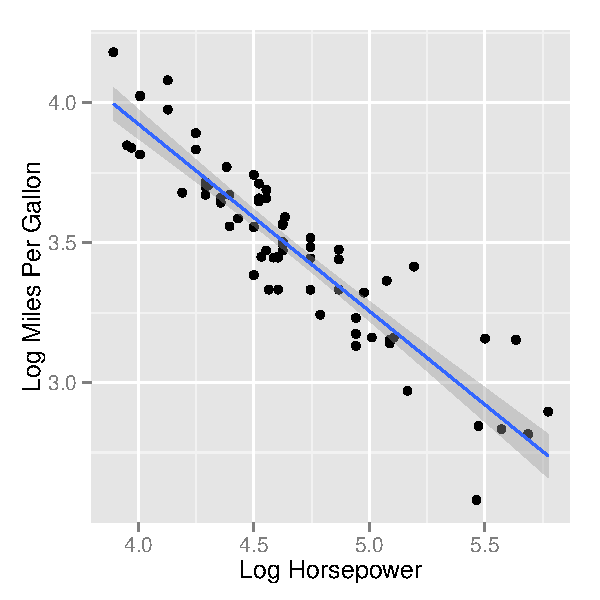
\includegraphics[width=\maxwidth]{figure/1bplot-1} 

}



\end{knitrout}

Residuals of this linear regression model and a bootstrap sampling of the residuals are shown below.  Additionally, a plot of residuals and a Q-Q plot of norm quantities are shown.

\begin{knitrout}
\definecolor{shadecolor}{rgb}{0.969, 0.969, 0.969}\color{fgcolor}\begin{kframe}
\begin{alltt}
\hlkwd{par}\hlstd{(}\hlkwc{mfrow} \hlstd{=} \hlkwd{c}\hlstd{(}\hlnum{1}\hlstd{,}\hlnum{2}\hlstd{))}
\hlkwd{plot}\hlstd{(lm.logmpg.loghp,} \hlkwc{which} \hlstd{=} \hlnum{1}\hlstd{)}
\hlkwd{abline}\hlstd{(}\hlkwc{h} \hlstd{=} \hlnum{0}\hlstd{,} \hlkwc{col} \hlstd{=} \hlstr{"gray75"}\hlstd{)}

\hlkwd{qqPlot}\hlstd{(lm.logmpg.loghp}\hlopt{$}\hlstd{residuals,} \hlkwc{las} \hlstd{=} \hlnum{1}\hlstd{,} \hlkwc{id.n} \hlstd{=} \hlnum{3}\hlstd{,}
       \hlkwc{ylab} \hlstd{=} \hlstr{"Residuals"}\hlstd{)}
\end{alltt}
\begin{verbatim}
## 82 72 55 
##  1 82 81
\end{verbatim}
\end{kframe}

{\centering 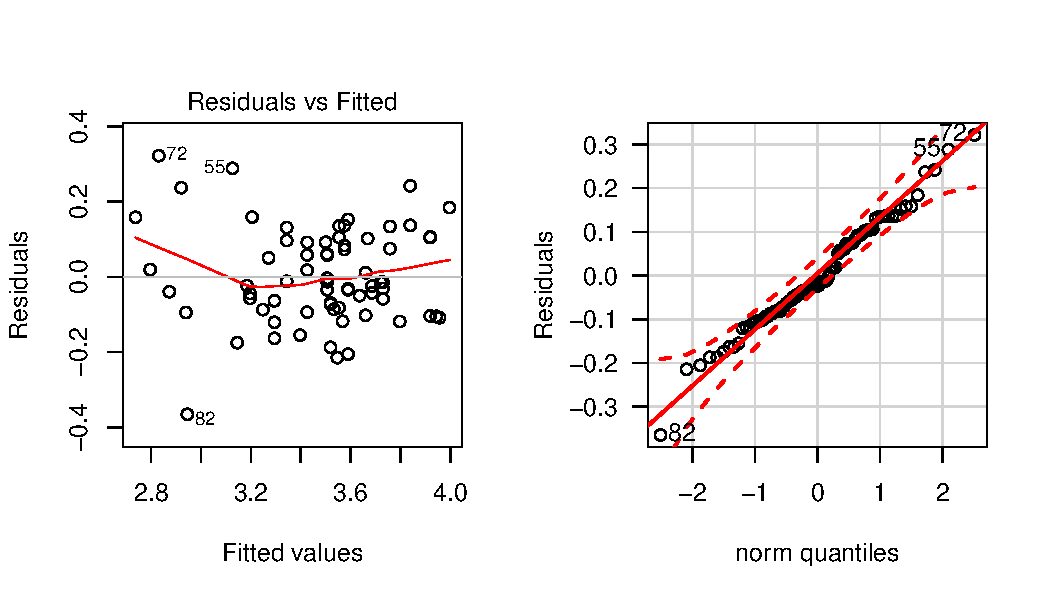
\includegraphics[width=\maxwidth]{figure/1b1-1} 

}



\end{knitrout}
Interpretation of Residuals:
\begin{itemize}
%  \item Based on the bootstrap distribution, the residuals appear to be normally distributed.
 \item There does not appear to be curvature associated with the residual plots.  From this observation, the quality of the fit does not vary with the independent variable (log(horsepower)).
 \item No obvious outliers exist.
 \item The Q-Q plot does not highlight any skewness in the resdiuals.
 \item No obvious pattern for the residuals exists.
\end{itemize}
Based on these observations, the residuals appear random and normally distributed.

\subsection{(5 pts) Investigate the leverages and Cook’s D. Use the 3p/n cutoff for large leverages, and the cutoff of 1 for large Cook’s D values. }

\begin{knitrout}
\definecolor{shadecolor}{rgb}{0.969, 0.969, 0.969}\color{fgcolor}\begin{kframe}
\begin{alltt}
\hlkwd{par}\hlstd{(}\hlkwc{mfrow}\hlstd{=}\hlkwd{c}\hlstd{(}\hlnum{1}\hlstd{,}\hlnum{3}\hlstd{))}
\hlkwd{plot}\hlstd{(lm.logmpg.loghp,}\hlkwc{which} \hlstd{=} \hlkwd{c}\hlstd{(}\hlnum{4}\hlstd{,}\hlnum{6}\hlstd{))}
\hlkwd{plot}\hlstd{(}\hlkwd{influence}\hlstd{(lm.logmpg.loghp)}\hlopt{$}\hlstd{hat,} \hlkwc{ylab} \hlstd{=} \hlstr{"Influence"}\hlstd{)}
\end{alltt}
\end{kframe}

{\centering 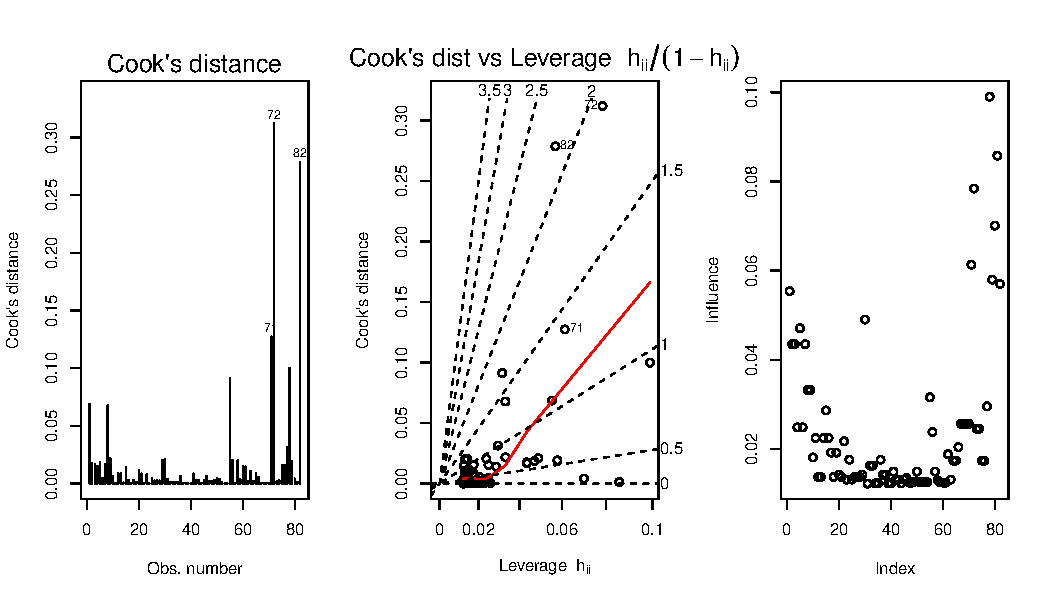
\includegraphics[width=\maxwidth]{figure/1c1-1} 

}



\end{knitrout}

Plots of Cook's distance, leverage versus Cook's distance, and influence / leverage are shown above.  Based on these visual analyses, no residual has a Cook's distance greater than 1, but three residual values have large leverages based on the 3p/n cutoff (leverage of 0.74).  No Values have both a Cook's distance greater than one and a leverage greater than 3p/n; therefore I do not think any observations have undue influence on the model fit.

\subsection{(10 pts) Assuming the model fits well, present and interpret the ANOVA table and R2 value.}
\begin{knitrout}
\definecolor{shadecolor}{rgb}{0.969, 0.969, 0.969}\color{fgcolor}\begin{kframe}
\begin{alltt}
\hlstd{mpg.anova} \hlkwb{<-} \hlkwd{anova}\hlstd{(lm.logmpg.loghp)}
\hlstd{mpg.anova}
\end{alltt}
\begin{verbatim}
## Analysis of Variance Table
## 
## Response: log_mpg
##           Df Sum Sq Mean Sq F value    Pr(>F)    
## log_hp     1 6.2780  6.2780  409.68 < 2.2e-16 ***
## Residuals 80 1.2259  0.0153                      
## ---
## Signif. codes:  0 '***' 0.001 '**' 0.01 '*' 0.05 '.' 0.1 ' ' 1
\end{verbatim}
\begin{alltt}
\hlstd{f.crit} \hlkwb{<-} \hlkwd{qf}\hlstd{(}\hlnum{1} \hlopt{-} \hlnum{0.05}\hlopt{/}\hlnum{2}\hlstd{, mpg.anova[}\hlnum{1}\hlstd{,}\hlnum{1}\hlstd{], mpg.anova[}\hlnum{2}\hlstd{,}\hlnum{1}\hlstd{])}
\hlstd{f.crit}
\end{alltt}
\begin{verbatim}
## [1] 5.218354
\end{verbatim}
\end{kframe}
\end{knitrout}

% latex table generated in R 3.1.0 by xtable 1.7-4 package
% Tue Dec  2 22:56:03 2014
\begin{table}[ht]
\centering
\begin{tabular}{r|ccccc}
  \hline
 & Df & Sum Sq & Mean Sq & F value & Pr($>$F) \\ 
  \hline
log\_hp & 1.000 & 6.278 & 6.278 & 409.682 & 0.000 \\ 
  Residuals & 80.000 & 1.226 & 0.015 &  &  \\ 
   \hline
\end{tabular}
\end{table}


The ANOVA F-test may be used to determine if $\beta_1$ (slope of regression line) is equal to zero; i.e., the mileage is not related to horsepower.  That is, $H_0 : \beta_1 = 0$ against the alternative $H_A : \beta_1 \ne 0$.  Because the F value of 410 is much larger than the critical F value of 5.2 and because the p-value is much less than 0.05, I reject the null hypothesis in favor of the alternative.  That is, the variation of mileage is related to vehicle horsepower.  The Sum of Squares divided by the degrees of freedom for the residuals ($s^2_{X|Y}$) was 0.015.

The $R^2$ value for the linear model was 0.837, which indicates that 83.7\% of the variation of mileage can be explained by variation of horsepower.

\subsection{(10pts) Present the parameter estimate table and estimated regression equation. State what the hypothesis test is related to the log(hp) line in the parameter estimate table. State the conclusion
of the hypothesis test. Interpret the slope coeffcient in the context of the model.}

\begin{knitrout}
\definecolor{shadecolor}{rgb}{0.969, 0.969, 0.969}\color{fgcolor}\begin{kframe}
\begin{alltt}
\hlstd{coef} \hlkwb{<-} \hlstd{sum.lm.logmpg.loghp}\hlopt{$}\hlstd{coefficients}
\end{alltt}
\end{kframe}
\end{knitrout}

Parameter Estimate Table:

% latex table generated in R 3.1.0 by xtable 1.7-4 package
% Tue Dec  2 22:56:03 2014
\begin{table}[ht]
\centering
\begin{tabular}{r|cccc}
  \hline
 & Estimate & Std. Error & t value & Pr($>$$|$t$|$) \\ 
  \hline
(Intercept) & 6.599 & 0.155 & 42.598 & 0.000 \\ 
  log\_hp & -0.669 & 0.033 & -20.241 & 0.000 \\ 
   \hline
\end{tabular}
\end{table}


Estimated Regression Equation:  $\text{log(Mileage)} = -0.699 * \text{log(Horsepower)} + 6.599$.  That is, $b_0 = 6.599$ and $b_1 = -0.699$.
\bigskip

Hypothesis tests of the regression equation parameters $\beta_0$ (intercept) and $\beta_1$ (slope) both have a null hypothesis that these values are equal to zero.  That is, $H_0: \beta_0 = 0$ and $H_0: \beta_1 = 0$ with the alternative $H_A: \beta_0 \text{ and } \beta_1 \ne 0$.

\bigskip

Slope of the regression line indicates that for every one unit of increase in log(Horsepower) the log(Mileage) will decrease by 0.699.

\subsection{(5pts) Using the R2 statistic and the slope of the regression line, what is the correlation between
log(hp) and log(mpg)?}
As was done previously:
the $R^2$ value for the linear model was 0.837, which indicates that 83.7\% of the variation of mileage can be explained by variation of horsepower.
The estimated regressioneEquation is:  $\text{log(Mileage)} = -0.699 * \text{log(Horsepower)} + 6.599$.  That is, $b_0 = 6.599$ and $b_1 = -0.699$.

\section{Gas Mileage and Automobile Weight}
\subsection{}

\begin{knitrout}
\definecolor{shadecolor}{rgb}{0.969, 0.969, 0.969}\color{fgcolor}\begin{kframe}
\begin{alltt}
\hlcom{# plot mpg = f(wt)}
\hlstd{p2a} \hlkwb{<-} \hlkwd{ggplot}\hlstd{(cars,} \hlkwd{aes}\hlstd{(}\hlkwc{x} \hlstd{= wt,} \hlkwc{y} \hlstd{= mpg))}
\hlstd{p2a} \hlkwb{<-} \hlstd{p2a} \hlopt{+} \hlkwd{geom_point}\hlstd{()}
\hlstd{p2a} \hlkwb{<-} \hlstd{p2a} \hlopt{+} \hlkwd{labs}\hlstd{(}\hlkwc{y} \hlstd{=} \hlstr{"Miles Per Gallon"}\hlstd{,} \hlkwc{x} \hlstd{=} \hlstr{"Weight"}\hlstd{)}
\hlstd{p2a} \hlkwb{<-} \hlstd{p2a} \hlopt{+} \hlkwd{geom_smooth}\hlstd{(}\hlkwc{method} \hlstd{= lm)}

\hlstd{p2b} \hlkwb{<-} \hlkwd{ggplot}\hlstd{(cars,} \hlkwd{aes}\hlstd{(}\hlkwc{x} \hlstd{= log_wt,} \hlkwc{y} \hlstd{= log_mpg))}
\hlstd{p2b} \hlkwb{<-} \hlstd{p2b} \hlopt{+} \hlkwd{geom_point}\hlstd{()}
\hlstd{p2b} \hlkwb{<-} \hlstd{p2b} \hlopt{+} \hlkwd{labs}\hlstd{(}\hlkwc{y} \hlstd{=} \hlstr{"Log Miles Per Gallon"}\hlstd{,} \hlkwc{x} \hlstd{=} \hlstr{"Log Weight"}\hlstd{)}
\hlstd{p2b} \hlkwb{<-} \hlstd{p2b} \hlopt{+} \hlkwd{geom_smooth}\hlstd{(}\hlkwc{method} \hlstd{= lm)}

\hlkwd{grid.arrange}\hlstd{(p2a, p2b,} \hlkwc{ncol} \hlstd{=} \hlnum{2}\hlstd{)}
\end{alltt}
\end{kframe}

{\centering 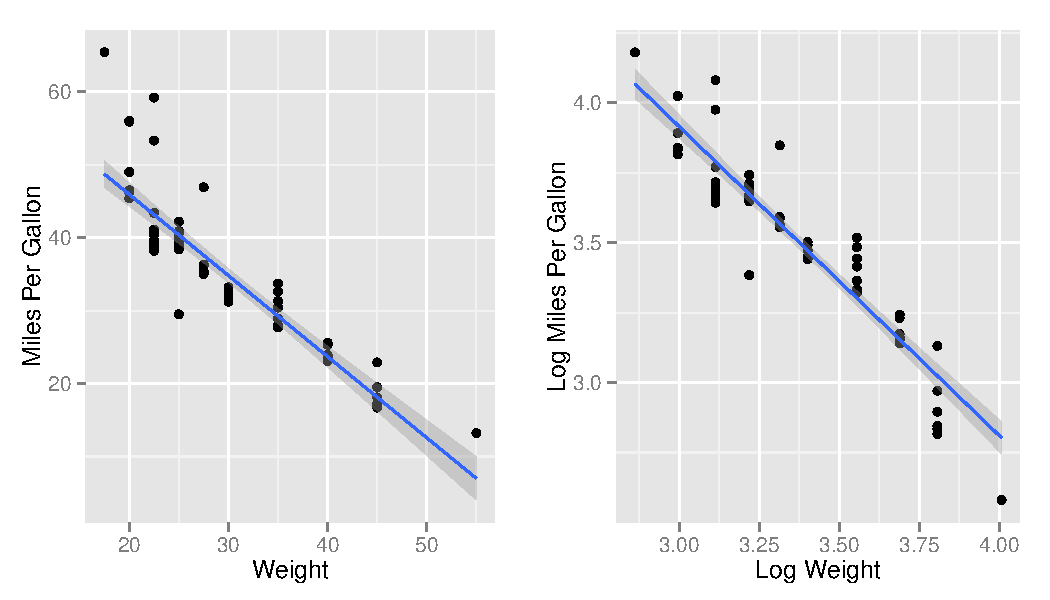
\includegraphics[width=\maxwidth]{figure/2a-1} 

}



\end{knitrout}

Based on these plots, little to no improvement in a linear fit would be gained from a log transformation of the data.  The linear model appears to fit both data sets equally well.
\subsection{}
\begin{knitrout}
\definecolor{shadecolor}{rgb}{0.969, 0.969, 0.969}\color{fgcolor}\begin{kframe}
\begin{alltt}
\hlcom{# Weight vs Mileage}
\hlstd{lm.mpg.wt} \hlkwb{<-} \hlkwd{lm}\hlstd{(mpg} \hlopt{~} \hlstd{wt,} \hlkwc{data} \hlstd{= cars)}
\hlstd{sum.lm.mpg.wt} \hlkwb{<-} \hlkwd{summary}\hlstd{(lm.mpg.wt)}
\hlkwd{summary}\hlstd{(lm.mpg.wt)}
\end{alltt}
\begin{verbatim}
## 
## Call:
## lm(formula = mpg ~ wt, data = cars)
## 
## Residuals:
##      Min       1Q   Median       3Q      Max 
## -10.8601  -2.2698  -1.1768   0.4899  16.6983 
## 
## Coefficients:
##             Estimate Std. Error t value Pr(>|t|)    
## (Intercept) 68.16545    1.86695   36.51   <2e-16 ***
## wt          -1.11222    0.05842  -19.04   <2e-16 ***
## ---
## Signif. codes:  0 '***' 0.001 '**' 0.01 '*' 0.05 '.' 0.1 ' ' 1
## 
## Residual standard error: 4.281 on 80 degrees of freedom
## Multiple R-squared:  0.8192,	Adjusted R-squared:  0.8169 
## F-statistic: 362.4 on 1 and 80 DF,  p-value: < 2.2e-16
\end{verbatim}
\begin{alltt}
\hlkwd{par}\hlstd{(}\hlkwc{mfrow} \hlstd{=} \hlkwd{c}\hlstd{(}\hlnum{1}\hlstd{,}\hlnum{2}\hlstd{))}
\hlkwd{plot}\hlstd{(lm.mpg.wt,} \hlkwc{which} \hlstd{=} \hlnum{1}\hlstd{)}
\hlkwd{abline}\hlstd{(}\hlkwc{h} \hlstd{=} \hlnum{0}\hlstd{,} \hlkwc{col} \hlstd{=} \hlstr{"gray75"}\hlstd{)}

\hlkwd{qqPlot}\hlstd{(lm.mpg.wt}\hlopt{$}\hlstd{residuals,} \hlkwc{las} \hlstd{=} \hlnum{1}\hlstd{,} \hlkwc{id.n} \hlstd{=} \hlnum{3}\hlstd{,}
       \hlkwc{ylab} \hlstd{=} \hlstr{"Residuals"}\hlstd{)}
\end{alltt}
\end{kframe}

{\centering 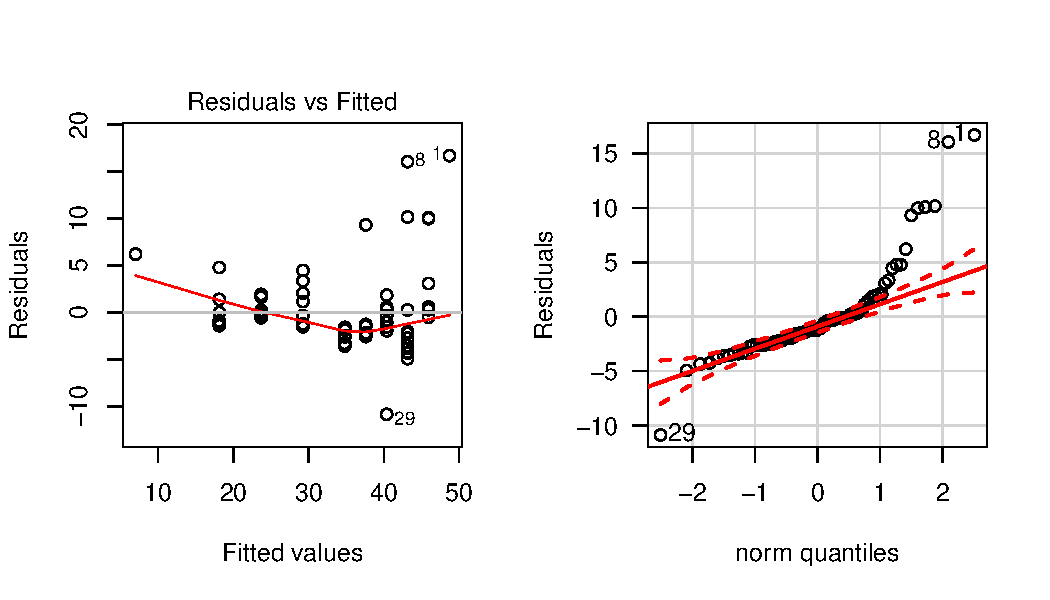
\includegraphics[width=\maxwidth]{figure/2b-1} 

}


\begin{kframe}\begin{verbatim}
##  1  8 29 
## 82 81  1
\end{verbatim}
\end{kframe}
\end{knitrout}

% latex table generated in R 3.1.0 by xtable 1.7-4 package
% Tue Dec  2 22:56:03 2014
\begin{table}[ht]
\centering
\begin{tabular}{r|cccc}
  \hline
 & Estimate & Std. Error & t value & Pr($>$$|$t$|$) \\ 
  \hline
(Intercept) & 68.165 & 1.867 & 36.512 & 0.000 \\ 
  wt & -1.112 & 0.058 & -19.037 & 0.000 \\ 
   \hline
\end{tabular}
\end{table}


\begin{knitrout}
\definecolor{shadecolor}{rgb}{0.969, 0.969, 0.969}\color{fgcolor}\begin{kframe}
\begin{alltt}
\hlkwd{shapiro.test}\hlstd{(sum.lm.mpg.wt}\hlopt{$}\hlstd{residuals)}
\end{alltt}
\begin{verbatim}
## 
## 	Shapiro-Wilk normality test
## 
## data:  sum.lm.mpg.wt$residuals
## W = 0.8019, p-value = 3.94e-09
\end{verbatim}
\begin{alltt}
\hlkwd{library}\hlstd{(nortest)}
\hlkwd{ad.test}\hlstd{(sum.lm.mpg.wt}\hlopt{$}\hlstd{residuals)}
\end{alltt}
\begin{verbatim}
## 
## 	Anderson-Darling normality test
## 
## data:  sum.lm.mpg.wt$residuals
## A = 5.443, p-value = 1.523e-13
\end{verbatim}
\end{kframe}
\end{knitrout}

Based on both the Shapiro-Wilks and Anderson-Darling tests for normality and the Q-Q plot, the residuals are not normally distributed.  Also, the residual variance appears to increase in relationship to vehicle weight.
\subsection{}

\begin{knitrout}
\definecolor{shadecolor}{rgb}{0.969, 0.969, 0.969}\color{fgcolor}\begin{kframe}
\begin{alltt}
\hlkwd{par}\hlstd{(}\hlkwc{mfrow}\hlstd{=}\hlkwd{c}\hlstd{(}\hlnum{1}\hlstd{,}\hlnum{3}\hlstd{))}
\hlkwd{plot}\hlstd{(lm.logmpg.loghp,}\hlkwc{which} \hlstd{=} \hlkwd{c}\hlstd{(}\hlnum{4}\hlstd{,}\hlnum{6}\hlstd{))}
\hlkwd{plot}\hlstd{(}\hlkwd{influence}\hlstd{(lm.logmpg.loghp)}\hlopt{$}\hlstd{hat,} \hlkwc{ylab} \hlstd{=} \hlstr{"Influence"}\hlstd{)}
\end{alltt}
\end{kframe}

{\centering 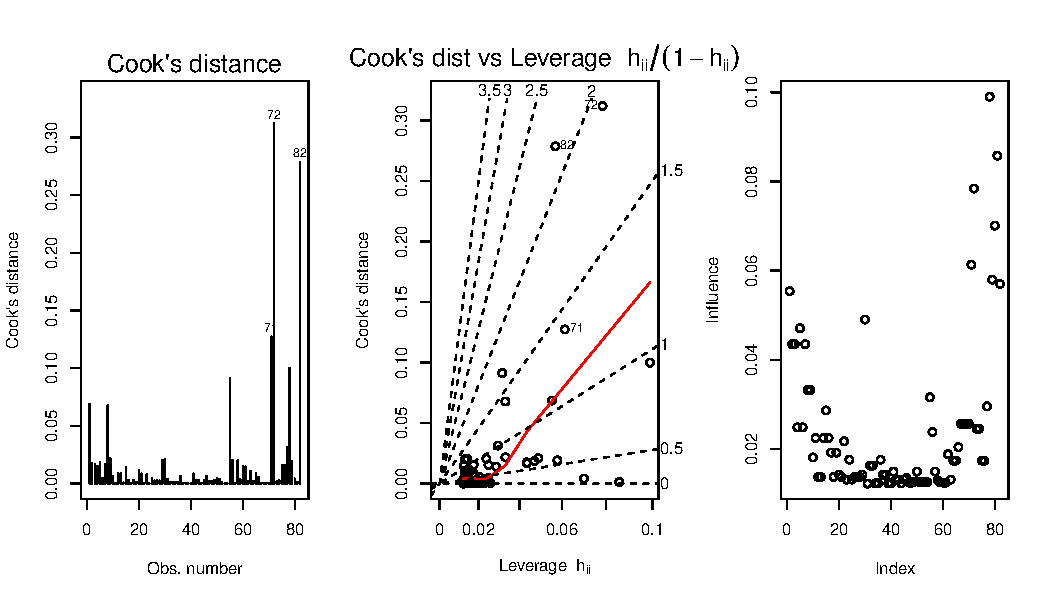
\includegraphics[width=\maxwidth]{figure/3b1-1} 

}



\end{knitrout}

Based on the leverage cuttoff and Cook's distance, no single point appears to have undue influence on the regression model.

\subsection{}
A weighted least squares model could be implemented to address the nonconstant variance of the residuals.  Also, a fit to a second order polynomial could be used instead of a straight-line model.  This seems reasonable, because the straight-line fit predicts that when you have a vehicle of zero weight the mileage will be 68 mpg, where intuitively I would interpret the mileage would assymptote to infinitely as vehicle weight approaches zero.
\end{document}
